% Nome del file: NormeDiProgetto.tex
% Percorso: Documenti\Interni\NormeDiProgetto\
% Autore: Vault-Tech
% Data creazione: 24.12.2015
% E-mail: vaulttech.swe@gmail.com
%
% Diario delle modifiche: interno al file.

\documentclass[a4paper, titlepage]{article}

\usepackage[margin=3cm]{geometry}
\usepackage{../../Stile}
\usepackage{../../Comandi}

\setcounter{secnumdepth}{5}
\setcounter{tocdepth}{5}

\def\NOME{Norme di Progetto}
\def\VERSIONE{1.0}
\def\DATA{31.12.2015}
\def\REDATTORE{Giacomo Beltrame \\ & Filippo Tesser}
\def\VERIFICATORE{Michela De Bortoli \\ & Miki Violetto}
\def\RESPONSABILE{Vassilikì Menarin}
\def\USO{Interno}
\def\DISTRIBUZIONE{\AUTORE}
%\def\SOMMARIO{Questo documento elenca le norme che i membri del \gl{team} Vault-Tech devono seguire durante lo sviluppo del progetto \CAPITOLATO.}

\begin{document}
\pagestyle{fancy}	
\pagenumbering{Roman}
\rfoot{Pagina \thepage{} di \pageref{lastromanpage}}

\maketitle

\begin{diario}
	\recap{Approvazione documento}{Filippo Tesser}{Responsabile}{03.03.2016}{3.0}
	\recap{Verifica del documento}{Simone Boccato}{Verificatore}{02.03.2016}{2.5}
	\recap{Correzione errori segnalati}{Giacomo Beltrame}{Amministratore}{01.03.2016}{2.4}
	\recap{Verifica del documento}{Simone Boccato}{Verificatore}{01.03.2016}{2.3}
	\recap{Incremento del documento}{Giacomo Beltrame}{Amministratore}{28.02.2016}{2.2}
	\recap{Stesura sezione dei test}{Giacomo Beltrame}{Amministratore}{26.02.2016}{2.1}
	\recap{Approvazione documento}{Miki Violetto}{Responsabile}{20.02.2016}{2.0}
	\recap{Verifica documento}{}{Michela De Bortoli}{19.02.2016}{1.2}
	\recap{Revisione correttiva dei contenuti}{Vassilikì Menarin}{Amministratore}{18.02.2016}{1.1}
	\recap{Approvazione documento}{Vassilikì Menarin}{Responsabile}{31.12.2015}{1.0}
	\recap{Correzione errori}{Filippo Tesser}{Amministratore}{31.12.2015}{0.9}
	\recap{Verifica documento}{Miki Violetto}{Verificatore}{30.12.2015}{0.8}
	\recap{Stesura sezione processi organizzativi}{Filippo Tesser}{Amministratore}{29.12.2015}{0.7}
	\recap{Stesura paragrafo Tracker}{Giacomo Beltrame}{Amministratore}{29.12.2015}{0.6}
	\recap{Aggiornamento della struttura del documento}{Filippo Tesser}{Amministratore}{28.12.2015}{0.5}
	\recap{Stesura sottosezione processi di verifica}{Giacomo Beltrame}{Amministratore}{28.12.2015}{0.4}
	\recap{Stesura sezione processi di supporto}{Filippo Tesser}{Amministratore}{27.12.2015}{0.3}
	\recap{Stesura sezione processi primari}{Filippo Tesser}{Amministratore}{26.12.2015}{0.2}	
	\recap{Stesura della struttura del documento}{Filippo Tesser}{Amministratore}{24.12.2015}{0.1}
\end{diario}

\newpage
\tableofcontents

\newpage
\listoffigures \label{lastromanpage}

\newpage
\clearpage
\pagenumbering{arabic}
\rfoot{Pagina \thepage{} di \pageref*{LastPage}}
\hypersetup{linkcolor=blue}

\section{Introduzione}
\subsection{Scopo del Documento}
In tale documento verranno definite le norme che i componenti del \gl{team} Vault-Tech dovranno seguire nello sviluppo del progetto, inoltre saranno indicati gli strumenti e le procedure da utilizzare.

La lettura del documento e l'adozione delle norme stilate è quindi necessaria da parte di tutti i membri per ottenere massima coerenza e efficienza durante lo svolgimento delle attività.

In particolar modo verranno trattate:
\begin{itemize}
	\item le interazioni tra i membri del \gl{team};
	\item le interazioni con entità esterne al \gl{team};
	\item la definizione dei ruoli e l'identificazione delle mansioni relative;
	\item le modalità di lavoro durante le varie fasi del progetto;
	\item le convenzione tipografiche nella stesura dei documenti;
	\item l'ambiente di sviluppo.
\end{itemize}

\subsection{Scopo del prodotto}
\SCOPO

\subsection{Glossario}
\GLOSSARIO

\subsection{Riferimenti}

%\subsubsection{Normativi}
%\begin{itemize}
%	\item \textbf{\iso{ISO 8601}}: \\gl{url}{http://en.\gl{wikipedia}.org/wiki/ISO\_8601};
%	\item \textbf{\iso{SI/ISO 31-0}}: \\gl{url}{http://en.\gl{wikipedia}.org/wiki/ISO\_31-0}.
%\end{itemize}

\subsubsection{Informativi}
\begin{itemize}
	\item \textbf{Guida utilizzo \gl{Git}}: \url{https://www.atlassian.com/git/tutorials/};
	\item \textbf{Gitflow Workflow}: \url{https://www.atlassian.com/git/tutorials/comparing-workflows/gitflow-workflow};
	\item \textbf{GNU AGPLv3}: \url{http://www.gnu.org/licenses/agpl-3.0.html}.
\end{itemize}

\newpage

\section{Processi primari}

\subsection{Processo di fornitura}
A seguire sono riportati gli standard coi quali il \gl{team} deve affrontare le attività di progetto.


\subsubsection{Attività}

\myparagraph{Studio di Fattibilità}
È il primo documento da redigere per la revisione dei requisiti.

Il \italics{Responsabile} deve organizzare delle riunioni con lo scopo di valutare gli altri capitolati. Gli esiti di tali riunioni saranno la base per la stesura dello \doc{Studio di Fattibilità} basato su:
\begin{itemize}
	\item \textbf{dominio tecnologico e applicativo}: conoscenza delle tecnologie richieste ed esperienze precedenti con problematiche poste dal capitolato;
	\item \textbf{rapporto costi/benefici}: prodotti simili già presenti sul mercato, quantità di requisiti obbligatori, costi in rapporto ai risultati previsti;
	\item \textbf{individuazione dei rischi}: comprensione dei punti critici della realizzazione quali mancanza di conoscenze o competenze e difficoltà nell'individuazione dei requisiti.
\end{itemize}

\subsection{Processi di sviluppo}

\subsubsection{Attività}

\myparagraph{Analisi dei Requisiti}
Terminata la stesura dello \doc{Studio di Fattibilità} è compito degli \italics{Analisti} redigere il documento \doc{Analisi dei Requisiti}. Questo documento ha il fine di raccogliere in modo sintetico e strutturato tutti i requisiti tratti da più fonti, quali: 
\begin{itemize}
	\item capitolato d'appalto;
	\item verbali di riunioni interne o esterne;
	\item casi d'uso.
\end{itemize}

Per tale scopo il \gl{team} ha sviluppato una piattaforma \gl{web}-based con cui elencare i requisiti e le loro dipendenze: \gl{Tracker}.

\myparagraph{Specifica Tecnica}
Questo documento verrà redatto dai \italics{Progettisti} e ha il compito di descrivere l'architettura del prodotto. Inoltre saranno progettati opportuni test di integrazione atti a individuare i problemi che si verificano quando due unità si combinano.
I seguenti diagrammi UML devono essere realizzati:
\begin{itemize}
	\item diagrammi delle classi;
	\item diagrammi dei package;
	\item diagrammi di attività;
	\item diagrammi di sequenza.
\end{itemize}
Infine devono essere descritti i vari design pattern che verranno utilizzati e il tracciamento requisito-componente atto a controllare lo stato di avanzamento del progetto.

\subsubsection{Procedure}

\myparagraph{Classificazione dei requisiti}
Ogni requisito individuato durante l'\doc{Analisi dei Requisiti} deve necessariamente, per questioni di tracciabilità, essere univocamente identificato con una stringa nel formato:
\centra{R[importanza][tipo][codice]}
dove:
\begin{itemize}
\item \textbf{importanza} può assumere i seguenti valori:
	\begin{itemize}
	\item O: \gl{requisito obbligatorio};
	\item D: \gl{requisito desiderabile};
	\item Z: \gl{requisito opzionale}.
	\end{itemize}
\item \textbf{tipo} può assumere i seguenti valori:
	\begin{itemize}
	\item F: requisito funzionale;
	\item Q: requisito qualitativo;
	\item P: requisito prestazionale;
	\item V: requisito vincolante.
	\end{itemize}
\item \textbf{codice} è il codice numerico gerarchico univoco.
\end{itemize}

Per ogni requisito sono inoltre specificati:
\begin{itemize}
\item una \textbf{descrizione} sintetica e non ambigua;
\item le \textbf{fonti} del requisito che possono essere uno o più elementi tra:
	\begin{itemize}
	\item capitolato d'appalto;
	\item verbale di riunioni interne o esterne;
	\item casi d'uso.
	\end{itemize}
\end{itemize}

\myparagraph{Classificazione dei casi d'uso}
Ogni caso d'uso individuato durante l'Analisi, analogamente ai requisiti, deve essere univocamente identificato con una stringa nel formato:
\centra{UC[codice]}
dove:
\begin{itemize}
\item \textbf{codice} è il codice numerico gerarchico univoco.
\end{itemize}

Inoltre per ogni caso d'uso sono specificati:
\begin{itemize}
\item \textbf{titolo}: un breve titolo riassuntivo;
\item \textbf{attori}: tutti gli attori coinvolti nel caso d'uso;
\item \textbf{scenario principale}: l'azione che l'attore compie perché la postcondizione sia raggiunta;
\item \textbf{scenari alternativi}: un elenco di decisioni che portano all'interruzione del normale flusso degli eventi;
\item \textbf{inclusioni}: elenco delle inclusioni se presenti;
\item \textbf{estensioni}: elenco delle estensioni se presenti;
\item \textbf{ereditarietà}: elenco dei casi d'uso eredi se presenti;
\item \textbf{descrizione}: una descrizione sintetica e completa del caso d'uso;
\item \textbf{precondizione}: le condizioni sempre vere all'origine del caso d'uso;
\item \textbf{postcondizione}: le condizioni sempre vere al termine del caso d'uso.
\end{itemize}

\myparagraph{Codifica e convenzioni}
Tutti i file contenente codice o documentazione \LaTeX{} devono essere conformi alla codifica \gl{UTF-8} con carattere di fine riga in stile \gl{Unix LF} e avere una riga vuota al termine.
Il codice deve seguire le linee guida Google reperibili all'indirizzo \url{https://github.com/google/styleguide}. I nomi delle variabili e classi deve essere in inglese, mentre i commenti in italiano.

\subsubsection{Strumenti}

\myparagraph{Tracker}
\gl{Tracker} è lo strumento sviluppato dal \gl{team} a supporto dell'attività di Analisi dei Requisiti. In particolare è stato dotato di una \gl{dashboard} che permette a tutti i membri del \gl{team} di mantenere sotto controllo le varie attività e la loro fase di avanzamento. Esso è inoltre in grado di redigere i documenti \doc{Analisi dei Requisiti} e \doc{Glossario} e di effettuare il tracciamento fonte-requisiti e requisiti-fonte grazie alla base di dati su cui poggia la logica del sistema. In futuro le sue funzionalità verranno estese per fornire ulteriori funzioni
di supporto per lo sviluppo del progetto e la stesura della successiva documentazione.

\newpage

\section{Processi di supporto}

\subsection{Processi di documentazione}
In queste sezioni verrà trattato il modello con il quale la documentazione viene prodotta.

\subsubsection{Procedure}

\myparagraph{Formalizzazione di un documento}
Per la formalizzazione di un documento è necessario il consenso del \italics{Responsabile}, in seguito al quale il documento può essere distribuito.
Nella seguente figura è illustrato il ciclo di vita di un documento.
\begin{figure}[!h]
	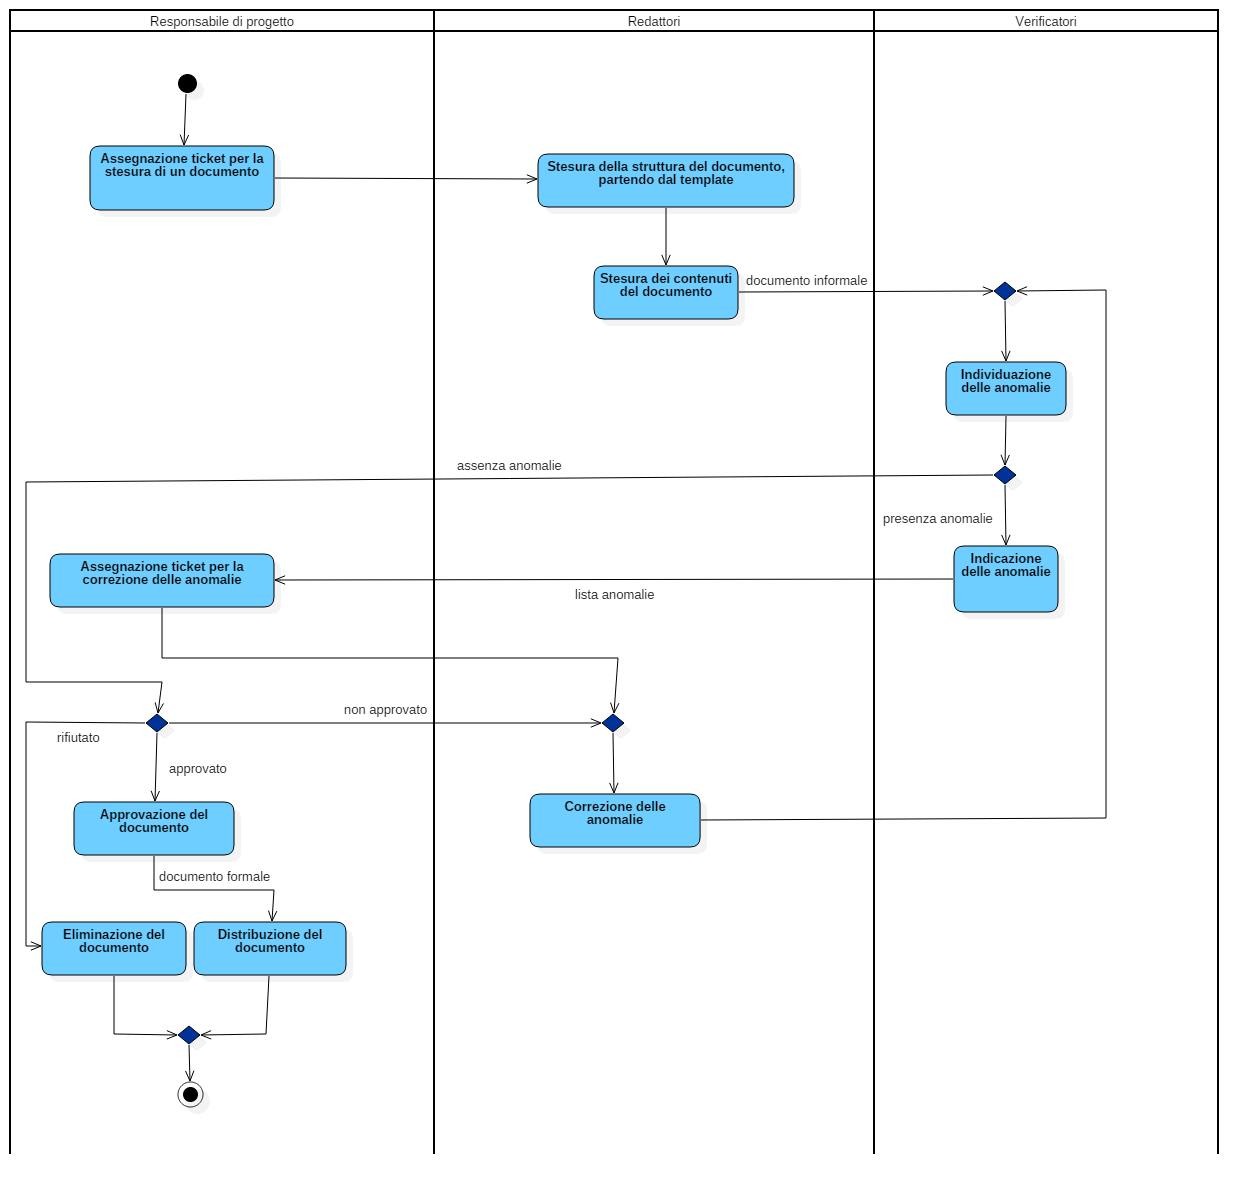
\includegraphics[width=\textwidth]{Img/docflow.png}
	\caption{Formalizzazione di un documento}
	\label{fig:documento}
\end{figure}
\newpage

\myparagraph{Template}
Ogni documento va realizzato a partire dal \gl{template} adatto, i \gl{template} sono disponibili ai membri del \gl{team} in una apposita directory su \gl{Google Drive} e nel \gl{repository} \gl{Github} del \gl{team}.
Nelle stesse directory sono presenti i file contenenti i comandi \LaTeX{} definiti dal \gl{team} necessari per compilare con successo i documenti.

\myparagraph{Norme tipografiche}
Qui sono elencate le condizioni di utilizzo di alcuni stili di testo e formato.

\mysubparagraph{Stile del testo}
\begin{description}
	\item[Grassetto] 
	Si utilizza solamente con lo scopo di dare enfasi ai termini o per evidenziare gli elementi di un elenco puntato.
	\item[Corsivo] 
	Si utilizza per i termini che sono voci del \doc{Glossario}, nomi di file, documenti e ruoli di progetto.
	\item[Monospace] 
	 Si utilizza per codice, comandi, percorsi e link \gl{URL}.
	 \item[G pedice]
	 I termini del \doc{Glossario} sono marcati in stile corsivo e con una G maiuscola a pedice.
	 \item[Maiuscolo]
	 Gli acronimi sono indicati completamente in maiuscolo. I nomi dei ruoli di progetto, dei documenti e altri termini importanti sono indicati solo con le iniziali maiuscole.
\end{description}

\mysubparagraph{Punteggiatura}
\begin{description}
	\item[Regola generale] 
	Ogni simbolo di punteggiatura non deve mai essere preceduto da un carattere di spaziatura ma solamente seguito. Non devono mai essere presenti più caratteri di spaziatura consecutivi.
	\item[Parentesi] 
	Le parentesi fanno eccezione alla regola generale poiché `(' o `[' devono essere precedute da spazio ma non seguite.
	\item[Virgolette singole] 
	Le virgolette singole vanno utilizzate per citare un singolo carattere (p.es. `g').
	\item[Virgolette doppie] 
	Le virgolette doppie racchiudono nomi di documenti o citazioni.
\end{description}

\mysubparagraph{Testo colorato}
Per link \gl{URL}, link che portano ad altre sezioni all'interno del documento e link mail, il testo è colorato in \crule[blue].

\mysubparagraph{Strutturazione delle sezioni}
La struttura delle sezioni dei documenti segue la formattazione standard di \LaTeX , a esclusione di \begin{verbatim}\paragraph e \subparagraph\end{verbatim} che sono stati ridefiniti in \begin{verbatim}\myparagraph e \mysubparagraph\end{verbatim} per motivi stilistici.

\mysubparagraph{Composizione del testo}
\begin{description}
	\item[Elenchi puntati] 
	Se l'elenco puntato è introdotto dai due punti `:', e prosegue quindi il discorso, allora ogni voce ha iniziale minuscola (acronimi, nomi di ruoli, nomi di fasi, ecc. fanno ovviamente eccezione). Ogni periodo è separato da punto e virgola `;'. L'ultima voce dell'elenco termina con un punto fermo `.'.
	
	Se invece l'elenco è di carattere descrittivo e non introdotto dai due punti, allora ogni voce ha iniziale maiuscola ed ogni periodo termina con un punto fermo.
	\item[Paragrafi] 
	I paragrafi sono tutti separati da una riga vuota.
	\item[Esempi] 
	Gli esempi vanno sempre indicati tra parentesi tonde e preceduti dall'abbreviazione ``es.''.
\end{description}

\mysubparagraph{Formati ricorrenti}
\begin{description}
	\item[Numeri] 
	Lo stile dei numeri deve aderire allo standard \iso{SI/ISO 31-0}.
	\item[Denaro] 
	Qualora sia necessario specificare una somma di denaro si deve far seguire al numero il simbolo `\euro' separato da uno spazio.
	\item[Date] 
	Lo stile delle date deve aderire al formato seguente:
	\centra{GG.MM.AAAA}
	dove:
	\begin{itemize}
		\item GG è il giorno in due cifre;
		\item MM è il mese in due cifre;
		\item AAAA è l'anno in quattro cifre.
	\end{itemize}
	\item[Orari] 
	Lo stile degli orari deve aderire allo standard \iso{ISO 8601} con il formato seguente:
	\centra{HH:MM}
	dove:
	\begin{itemize}
		\item HH è l'ora in due cifre;
		\item MM sono i minuti in due cifre.
	\end{itemize}
	\item[Luoghi] 
	Lo stile dell'indicazione di un luogo deve aderire al formato:
	\centra{Città (PR) in via Nome della Via, \#}.
	\item[Nomi propri di persona] 
	Il nome precede il cognome. Se la persona possiede un titolo noto che è necessario specificare esso va fatto precedere al nome con notazione minuscola e abbreviata (p.es. dott. Mario Rossi).
	\item[Sigle] 
	Le sigle dei documenti e delle revisioni potranno essere utilizzate solo nelle tabelle per questioni di spazio. In particolare sono previste le seguenti sigle:
	\begin{itemize}
		\item \textbf{NP}: Norme di Progetto;
		\item \textbf{Gl}: Glossario;
		\item \textbf{SF}: Studio di Fattibilità;
		\item \textbf{AR}: Analisi dei Requisiti;
		\item \textbf{PQ}: Piano di Qualifica;
		\item \textbf{PP}: Piano di Progetto;
		\item \textbf{ST}: Specifica Tecnica;
		\item \textbf{DP}: Definizione di Prodotto;
		\item \textbf{MU}: Manuale Utente;
		\item \textbf{RR}: Revisione dei Requisiti;
		\item \textbf{RP}: Revisione di Progettazione;
		\item \textbf{RQ}: Revisione di Qualifica;
		\item \textbf{RA}: Revisione di Accettazione.
	\end{itemize}
	\item[Nomi di documenti di progetto]
	Il nome di documenti del \gl{team} è indicato in corsivo, con iniziale maiuscola e tra doppie virgole.
	\item[Nomi di ruoli di progetto]
	Il nome di un ruolo del \gl{team} è indicato in corsivo, con iniziale maiuscola.
\end{description}

\myparagraph{Componenti grafiche}

\mysubparagraph{Immagini}
Le immagini da inserire nei documenti devono essere in formato \gl{PDF} o \gl{PNG}. Ogni immagine sarà corredata di numero progressivo e didascalia, riportati nell'indice delle figure.

\mysubparagraph{Tabelle}
Nella stesura delle tabelle sarà obbligatoria l'osservazione delle regole di seguito descritte, al fine di aumentarne la tracciabilità e la facilità di lettura.
\begin{description}
	\item[Titolo] 
	Ogni tabella dovrà essere descritta da un numero progressivo e un titolo riassumente i contenuti.
	\item[Intestazioni colonne] 
	L'intestazione conterrà i titoli delle colonne. Esse avranno \crule[I] come colore di sfondo e testo bianco.
	\item[Righe] 
	Le righe dovranno presentare colori di sfondo alterni tra \crule[P] e \crule[D].
	\item[Bordi] 
	Una linea verticale \crule[I] separa le colonne.
\end{description}

\myparagraph{Formattazione pagine}

\mysubparagraph{Copertina}
Sulla prima pagina del documento sono visibili centrati e in ordine dall'alto verso il basso:
\begin{itemize}
	\item il logo e nome del \gl{team};
	\item nome del progetto;
	\item titolo del documento comprensivo di versione;
%	\item breve sommario;
	\item tabella informativa del documento contenente:
	\begin{itemize}
		\item nome del documento privo di versione;
		\item versione del documento;
		\item data di approvazione del documento;
		\item nome e cognome dei redattori in ordine alfabetico per cognome;
		\item nome e cognome dei \italics{Verificatori} in ordine alfabetico per cognome;
		\item nome e cognome del \italics{Responsabile} che ha approvato il documento;
		\item uso (interno o esterno);
		\item lista di distribuzione.
	\end{itemize}
\end{itemize}

\mysubparagraph{Diario delle modifiche}
Dalla seconda pagina di ogni documento è visibile il diario delle modifiche. Ogni riga del diario delle modifiche contiene in ordine:
\begin{itemize}
	\item versione del documento prodotta dopo la modifica;
	\item un breve ma chiaro riepilogo delle modifiche svolte;
	\item nome e cognome dell'autore;
	\item ruolo dell'autore al momento della modifica;
	\item data della modifica.
\end{itemize}
La tabella è ordinata per versione in ordine decrescente.

\mysubparagraph{Indici}
In ogni documento, dopo il diario delle modifiche, è presente un indice rispettivamente per le sezioni, le figure e le tabelle.

\mysubparagraph{Intestazione}
L'intestazione di ogni pagina contiene:
\begin{itemize}
	\item logo e nome del gruppo;
	\item numero e titolo della sezione corrente.
\end{itemize}

\mysubparagraph{Piè di pagina}
A piè di pagina vengono indicati il nome e la versione del documento a sinistra, la email del \gl{team} al centro come link e la numerazione pagine a destra.

\mysubparagraph{Numerazione pagine}
La parte di copertina, indici e diario delle modifiche segue la numerazione in numeri romani.
La numerazione pagine del contenuto vero e proprio di ogni documento invece segue la classica numerazione in numeri arabi.
La numerazione adotta il seguente formato:
\centra{Pagina X di Y}
dove:
\begin{itemize}
	\item X è il numero di pagina corrente;
	\item Y il numero di pagine totali.
\end{itemize}


\myparagraph{Tipi di documento}

\mysubparagraph{Documenti preliminari}
Tutti i documenti sono preliminari dalla loro creazione fino all'approvazione da parte del \italics{Responsabile} ed il loro utilizzo è quindi destinato esclusivamente ad uso interno.

\mysubparagraph{Documenti formali}
Una volta avvenuta l'approvazione da parte del \italics{Responsabile} il documento viene ritenuto formale ed è quindi distribuibile ai soggetti presenti nella lista di distribuzione.

Ogni modifica effettuata produrrà una nuova versione del documento da considerarsi preliminare e rimarrà tale fino ad una successiva approvazione da parte del \italics{Responsabile}.

\mysubparagraph{Glossario}
\GLOSSARIO

\mysubparagraph{Verbali}
Dopo ogni riunione interna o esterna spetta al segretario verbalizzante redigere il documento. I verbali non sono soggetti a \gl{versionamento}. Il codice identificativo di ogni verbale segue la seguente struttura: 
\centra{V[data]} 
dove:
\begin{itemize}
	\item \textbf{data} è la data della riunione alla quale il verbale fa riferimento nel formato GG.MM.AAAA.
\end{itemize}

Ogni verbale dovrà presentare le seguenti informazioni nell'ordine in cui sono elencate:
\begin{itemize}
	\item data, ora e luogo della riunione;
	\item i presenti, gli assenti, il nome di chi presiede e quello del segretario verbalizzante;
	\item l'ordine del giorno;
	\item gli interventi più significativi presentati in ordine cronologico;
	\item le conclusioni e le decisioni assunte;
	\item i problemi irrisolti.
\end{itemize}


\myparagraph{Intestazione sorgenti documentazione}
Ogni file sorgente della documentazione deve essere intestato nel seguente modo:
\begin{lstlisting}[language=TeX,numbers=left]
% Nome del file: NormeDiProgetto.tex
% Percorso: /Documenti/Interni/NormeDiProgetto/
% Autore: Vault-Tech
% Data creazione: 24-12-2015
% E-mail: vaulttech.swe@gmail.com
% Diario delle modifiche: interno al file.
\end{lstlisting}

\myparagraph{Versionamento dei documenti}
Ogni documento presenta un numero di versione dopo il nome nel formato seguente:
\centra{vX.Y}
dove:
\begin{itemize}
	\item X è un numero intero incrementato di una unità in occasione di una formalizzazione, l'incremento di X porta Y a 0;
	\item Y è un numero intero incrementato ad ogni modifica effettuata sul documento e riportata nel diario delle modifiche.
\end{itemize}

\subsubsection{Strumenti}

\myparagraph{\LaTeX}
Per redigere i documenti viene utilizzato il \gl{linguaggio di markup} \LaTeX. La possibilità di definire delle variabili all'interno dei fogli di stile consente di automatizzare l'aggiornamento di tutti i riferimenti presenti all'interno dei diversi documenti.

\myparagraph{TeXstudio}
L'\gl{IDE} \gl{TeXstudio} è utilizzato per redigere la documentazione in \gl{linguaggio di markup} \LaTeX. Esso consente di effettuare il controllo ortografico automatico durante la digitazione del testo ed è inoltre multipiattaforma.

\myparagraph{Hunspell}
Per un ulteriore e più avanzata correzione di errori ortografici nei documenti si utilizza il tool \gl{Hunspell} v1.3.3.

\myparagraph{StarUML}
Per la realizzazione dei diagrammi \gl{UML} da inserire nei documenti viene usato il \gl{software} \gl{StarUML} 2.6.0, \gl{open source} e multipiattaforma.

\myparagraph{Redmine}
Per la realizzazione dei \gl{diagrammi di Gantt} da inserire nei documenti viene usato la funzione di creazione di diagrammi fornita da \gl{Redmine}. 

\myparagraph{Script}
Per alcune funzioni più avanzate e particolari sono disponibili degli \gl{script} creati dal \gl{team}, a seguire i principali e più utili:
\begin{itemize}
	\item \gl{script} per calcolare l'\gl{Indice Gulpease};
	\item \gl{script} di glossarizzazione automatica dei termini all'interno dei documenti.
\end{itemize}
Tali \gl{script} si trovano in una directory apposita nel \gl{repository}.

\newpage

\subsection{Processo di verifica}

\subsubsection{Attività}

\myparagraph{Analisi}

\mysubparagraph{Analisi statica}
L'analisi statica è un processo di verifica che consente di trovare le anomalie all'interno dei file di codice e documentazione. Le tecniche principali di analisi statica sono:
\begin{description}
	\item[\gl{Walkthrough}:] l'analisi \gl{walkthrough} viene utilizzata quando non si ha una lista che elenca le anomalie riscontrate in precedenza durante le attività di verifica, chiamata lista di controllo; questa analisi consiste nell'ispezione dell'intero file in cerca di violazioni delle norme e errori.
	\item[\gl{Inspection}:] l'analisi \gl{inspection} viene utilizzata quando si ha una lista di controllo e permette di fare una ricerca mirata degli errori e delle violazioni delle norme nel codice o nel documento.
\end{description}

\mysubparagraph{Analisi dinamica}
L'analisi dinamica può essere svolta solamente sulle componenti software ed è utile a evidenziare anomalie presenti nel codice. Vengono eseguiti dei test su parti di sistema per verificare che ognuna di esse produca il risultato desiderato. Prima di eseguire un qualsiasi test è necessario conoscere la precondizione e postcondizione del sistema per poterne decretare l'esito.

\myparagraph{Test}
Segue un elenco dei tipi di test che vengono effettuati.

\mysubparagraph{Test di unità}
Sono test atti a verificare che ogni singola unità di prodotto funzioni nel modo corretto. In questo tipo di test ogni componente del sistema viene verificata isolata dal resto del sistema.
Il codice identificativo dei test di unità è: \centra{TU[codice univoco]}.

\mysubparagraph{Test di integrazione}
I test di integrazione rappresentano l'estensione logica del test di unità. Il tipo più semplice di test di integrazione consiste nella combinazione di due unità già sottoposte a test in un solo componente e nel test dell'interfaccia presente tra le due. In uno scenario realistico più unità vengono combinate in componenti che, a loro volta, vengono aggregate in parti più grandi del sistema. Alla fine, tutti i moduli che compongono un processo vengono sottoposti al test contemporaneamente.
Il codice identificativo dei test di integrazione è: \centra{TI[IDcomponente]} dove IDcomponente rappresenta la componente i cui elementi integrati sono sottoposti al test. Qualora più componenti abbiano lo stesso nome identificativo verrà associato a IDcomponente anche la componente principale che possa identificarli in modo univoco (ad esempio TIServicesClient e TIServicesServer).

\mysubparagraph{Test di regressione}
Il test di regressione va eseguito ogni volta che viene modificata un'implementazione del sistema. A tale scopo, è possibile eseguire nuovamente i test esistenti sul codice modificato per stabilire se le modifiche apportate hanno alterato elementi precedentemente funzionanti. Se necessario è anche possibile scrivere nuovi test.

\mysubparagraph{Test di sistema}
Sono test che vengono eseguiti quando si pensa che il prodotto sia giunto a una versione definitiva. In sostanza si controlla che il sistema soddisfi tutti i requisiti.
Il codice identificativo dei test di sistema è: \centra{TS[CodiceRequisito]} dove CodiceRequisito identifica il codice univoco associato ad ogni requisito descritto nell'\doc{Analisi dei requisiti}.

\mysubparagraph{Test di validazione}
Questo tipo di test viene svolto durante la fase di collaudo antecedente il rilascio sotto supervisione del proponente. Si controlla che il sistema soddisfi almeno tutti i requisiti obbligatori. Se l'esito del test è positivo viene consentito il rilascio del prodotto.
Il codice identificativo per tale tipo di test è: \centra{TV[CodiceRequisito]} dove CodiceRequisito identifica il codice univoco associato ad ogni requisito descritto nell'\doc{Analisi dei requisiti}.

\subsubsection{Procedure}

\myparagraph{Gestione anomalie}
Alla risoluzione di ogni \gl{ticket} il \italics{Verificatore} deve procedere alla verifica dell'operato. Ogni anomalia individuata viene annotata all'interno di un elenco. L'elenco delle anomalie è comunicato al \italics{Responsabile} che si occupa di assegnare un \gl{ticket} per la correzione al responsabile di esse.

L'elenco delle anomalie riscontrate viene utilizzato per stilare una lista di controllo utile ai processi di verifica futuri. La segnalazione di una anomalia deve specificare il file oggetto della verifica, la posizione dell'anomalia all'interno del file, il suo tipo e la sua descrizione.


\newpage

\section{Processi organizzativi}

\subsection{Processo di gestione}

\subsubsection{Attività}

\myparagraph{Comunicazioni}

\mysubparagraph{Comunicazioni interne}
Le comunicazioni interne al \gl{team} avvengono tramite due piattaforme:
\begin{description}
	\item[\gl{Telegram}:] Applicazione di messaggistica utilizzata principalmente per questioni generali e organizzative del \gl{team}.
	\item[\gl{Slack}:] Applicazione che permette la divisione della chat in vari gruppi e la pubblicazione di messaggi automatici ad ogni aggiornamento del \gl{repository}.
\end{description}

\mysubparagraph{Comunicazioni esterne}
Per le comunicazioni esterne è stata creata la casella di posta elettronica: \centra{\bold{\EMAIL.}} Questa casella è l'unico canale di comunicazione con l'esterno ed è esclusivamente accessibile al \italics{Responsabile} che è quindi l'unico a poter comunicare con il committente del progetto. Sarà poi il \italics{Responsabile} a informare i membri del gruppo delle discussioni avvenute qualora lo ritenga opportuno.

Di seguito è spiegato il contenuto e la forma che una e-mail deve avere.
\begin{description}
	\item[Oggetto:] 
	L'oggetto deve essere descritto chiaramente, e non deve essere confondibile con altri preesistenti. Avviata una comunicazione, l'oggetto non deve essere mai cambiato. Deve essere aggiunta la particella ``Re:'' all'inizio dell'oggetto nel caso in cui si debba comporre una risposta. Se si tratta invece di un inoltro, si antepone ``I:'' all'oggetto.
	\item[Formula d'apertura:] 
	La formula d'apertura deve cominciare con un aggettivo di cortesia o un saluto e il nome del destinatario preceduto, se in possesso di un titolo noto, dall'abbreviazione del titolo stesso e terminare con una virgola (p.es. ``Gentile dott. Mario Rossi,'').
	\item[Corpo:] 
	Il corpo del messaggio deve essere chiaro e deve contenere tutte le informazioni necessarie a rendere comprensibile l'argomento trattato. È buona norma separare distintamente il corpo, con doppio ritorno a capo dalla formula di apertura. Se il corpo presenta più paragrafi vanno separati con una riga vuota. In caso di risposta o inoltro di una e-mail, il nuovo contenuto deve sempre essere in testa.
	\item[Formula di chiusura:] 
	La formula di chiusura è separata dal corpo con doppio ritorno a capo. Essa prevede il saluto più adatto alla conversazione seguito da una virgola e, dopo un ritorno a capo, la firma del mittente.
\end{description}


\newpage


\myparagraph{Riunioni}

\mysubparagraph{Riunioni interne}
Le riunioni interne al \gl{team} saranno fissate dal \italics{Responsabile} e sarà compito suo avvisare tutti i membri del \gl{team}. Qualunque membro del \gl{team} può richiedere la convocazione di una riunione interna inviando una richiesta al \italics{Responsabile} che deciderà se accettarla o respingerla. La convocazione verrà effettuata da quest'ultimo con almeno tre giorni di anticipo tramite il canale apposito nella piattaforma \gl{Slack}. La partecipazione dei membri ad esse sarà obbligatoria, salvo problematiche o impegni improrogabili personali.

\mysubparagraph{Riunioni esterne}
Le riunioni esterne, tenute con il committente o l'azienda proponente, saranno concordate dal \italics{Responsabile} che avviserà, con almeno tre giorni di preavviso, i membri del \gl{team} mediante il canale apposito nella piattaforma \gl{Slack}. Ogni membro del \gl{team} può richiedere un incontro, specificandone il motivo, al \italics{Responsabile} che deciderà se procedere a contattare la parte esterna.

\myparagraph{Ticketing}
Il sistema di ticketing permette di assegnare le mansioni ai vari membri del \gl{team} assegnandone la priorità e permettendo di impostarne lo stato. Ciò permette al \italics{Responsabile} di tenere sotto controllo l'avanzamento delle attività di progetto in ogni momento.

\myparagraph{Repository}
Per permettere la collaborazione e la condivisione dei file necessari allo sviluppo delle varie attività di progetto si è scelto di adottare un \gl{repository}. L'\gl{host} che si è scelto di utilizzare permette, con licenza ``Academic'', la creazione di un \gl{repository} privato, accessibile ai soli membri del \gl{team}.

L'\italics{Amministratore} si occupa di inserire i membri del \gl{team} tra i collaboratori al progetto.

\subsubsection{Procedure}

\myparagraph{Apertura e assegnazione di un ticket}
Il \italics{Responsabile} ha il compito di aprire e assegnare un \gl{ticket} a uno dei membri del \gl{team} attraverso l'applicativo \gl{Redmine}.

Devono essere specificati:
\begin{itemize}
	\item \textbf{tracker}: ``Formazione'', ``Pianificazione'', ``Analisi'', ``Codifica'', ``Verifica'', ``Correzione'' o ``Amministrazione'';
	\item \textbf{oggetto};
	\item \textbf{descrizione};
	\item \textbf{stato}: all'apertura il \gl{ticket} sarà obbligatoriamente in stato ``Aperto''; gli altri stati in cui un \gl{ticket} può trovarsi sono ``In elaborazione'', ``Sospeso'', ``Risolto'' o ``Abortito'';
	\item \textbf{priorità}: ``Bassa'', ``Normale'', ``Alta'', ``Urgente'', ``Immediata'';
	\item \textbf{assegnatario}: un membro del \gl{team};
	\item \textbf{branch}: specifica il branch del \gl{repository} sul quale lavorare per risolvere il \gl{ticket};
	\item \textbf{data di inizio}: il giorno in cui l'assegnatario può cominciare ad elaborare il \gl{ticket};
	\item \textbf{data di scadenza}: il giorno limite in cui il \gl{ticket} deve essere risolto per non causare ritardi.
\end{itemize}
Possono inoltre essere specificati uno o più osservatori dello stato di avanzamento del \gl{ticket} e/o allegare un file (p.es. l'elenco delle anomalie).

\myparagraph{Risoluzione di un ticket}
L'assegnatario di un \gl{ticket} può modificarne lo stato secondo le seguenti relazioni:
\begin{itemize}
	\item ``Aperto'' $\to$ ``In elaborazione'';
	\item ``In elaborazione'' $\to$ ``Sospeso'';
	\item ``Sospeso'' $\to$ ``In elaborazione'';
	\item ``In elaborazione'' $\to$ ``Risolto''.
\end{itemize}
Il \italics{Responsabile} può impostare lo stato di un \gl{ticket} ad ``Abortito'' in qualsiasi momento. Nel caso in cui un \gl{ticket} venga abortito mentre era in elaborazione l'assegnatario di tale \gl{ticket} dovrà sospendere immediatamente le attività correlate ad esso.
\newpage
A seguire sono riportate le procedure che portano alla risoluzione di un \gl{ticket}.
\begin{figure}[!h]
	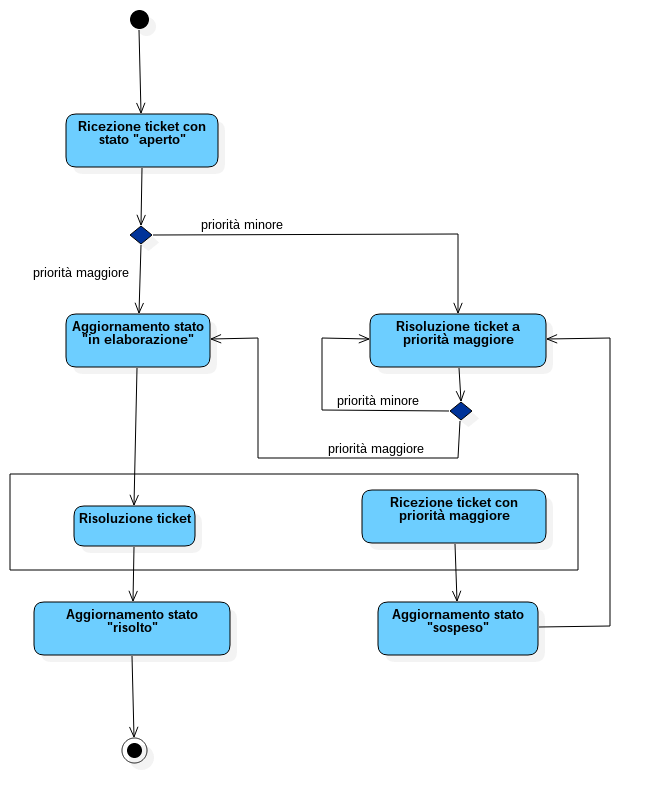
\includegraphics[width=\textwidth]{Img/flowticket.png}
	\caption{Risoluzione di \gl{ticket}}
	\label{fig:documento}
\end{figure}
\newpage

\subsubsection{Norme}

\myparagraph{Risorse}
Le risorse necessarie per la realizzazione del progetto, e quelle realmente disponibili, si dividono in tre principali categorie:
\mysubparagraph{Risorse umane}
\begin{itemize}
	\item \bold{Necessarie}
	\newline Le risorse umane necessarie per lo svolgimento di tale progetto in modo corretto e completo rispetto agli obiettivi di qualità sono gli individui di un \gl{team} che ricoprano tutti i seguenti ruoli:
	\begin{itemize}
		\item \italics{Responsabile}
		\item \italics{Amministratore}
		\item \italics{Analista}
		\item \italics{Progettista}
		\item \italics{Programmatore}
		\item \italics{Verificatore}
	\end{itemize}
	\ 
	\item \bold{Disponibili}
	\newline All'interno del gruppo di sviluppo sono disponibili sufficienti persone per ricoprire tutti i ruoli necessari all'esecuzione delle attività di verifica.
\end{itemize}

\mysubparagraph{Risorse software}
\begin{itemize}
	\item \bold{Necessarie}
	\newline Le risorse \gl{software} necessarie sono un sistema operativo possibilmente comune a tutti i membri del gruppo e gli strumenti che garantiscano la miglior qualità possibile nell'attuare le attività di verifica sui prodotti e sui processi. 
	\ 
	\item \bold{Disponibili}
	\newline  Si dispone del numero sufficiente di strumenti, installati e funzionanti, per svolgere le attività di verifica richieste in questo documento.
\end{itemize}

\mysubparagraph{Risorse hardware}
\begin{itemize}
	\item \bold{Necessarie}
	\newline Come risorse \gl{hardware} sono richiesti computer con sufficienti prestazioni su cui lavorare ed eseguire tutto il \gl{software} necessario durante le attività da svolgere.
	\ 
	\item \bold{Disponibili}
	\newline Ogni membro del gruppo dispone di un computer personale su cui lavorare; in caso di problemi il \gl{team} potrà usufruire dei computer forniti dal Servizio di Calcolo dell’Università degli Studi di Padova.
\end{itemize}

\myparagraph{Ruoli di progetto}
Lo sviluppo di un progetto prevede la collaborazione di individui a cui sono stati assegnati diversi ruoli. Tali ruoli rappresentano le omonime figure aziendali, indispensabili per il buon esito del progetto. Si garantisce che ogni componente del \gl{team} ricoprirà tutti i ruoli almeno una volta. A tal proposito, potrebbero sorgere delle problematiche relative a conflitti d’interesse (esempio: lo stesso soggetto potrebbe ritrovarsi a ricoprire un ruolo e, in seguito, a verificare l’operato svolto in precedenza). Queste situazioni non dovranno mai presentarsi poiché potrebbero ledere la qualità del prodotto. È quindi importante che le attività vengano pianificate con attenzione e che ciascun membro del \gl{team} assicuri l’esclusivo svolgimento del ruolo a lui assegnato. Nel corso del progetto i ruoli all'interno del gruppo ruoteranno come illustrato nel \doc{Piano di Progetto}. Al sorgere di eventuali incongruenze, si provvederà a notificare il \italics{Responsabile}, che avrà il compito di risolvere la questione.
Di seguito si discuterà dei vari ruoli, delle relative responsabilità e delle modalità operative.

\mysubparagraph{Responsabile}
Il \italics{Responsabile} rappresenta il progetto, in quanto accentra su di sé le responsabilità di scelta e di approvazione, e il \gl{team}, poiché presenta al committente i risultati del
lavoro svolto.
Detiene il potere decisionale, quindi la responsabilità in merito a:
\begin{itemize}
	\item pianificazione, coordinamento e controllo delle attività;
	\item gestione e controllo delle risorse;
	\item analisi e gestione dei rischi;
	\item approvazione dei documenti;
	\item approvazione dell'offerta economica.
\end{itemize}
Di conseguenza, ha il compito di:
\begin{itemize}
	\item assicurarsi che le attività di verifica e validazione vengano svolte sistematicamente in riferimento alle \doc{Norme di Progetto};
	\item garantire che vengano rispettati i ruoli e le competenze assegnate nel \doc{Piano di Progetto};
	\item garantire che non vi sia alcun conflitto tra redattori e verificatori.
\end{itemize}

\mysubparagraph{Amministratore}
L'\italics{Amministratore} è il responsabile dell'efficienza e del rendimento dell'ambiente lavorativo. Le mansioni che gli competono sono le seguenti:
\begin{itemize}
	\item ricercare strumenti che possano automatizzare il maggior numero possibile di compiti e operazioni;
	\item gestire l'archiviazione e il \gl{versionamento} della documentazione di progetto;
	\item controllare le versioni dei prodotti e gestire le configurazioni;
	\item fornire strumenti e procedure per la segnalazione ed il monitoraggio ai fini del controllo qualità;
	\item risolvere i problemi legati alle difficoltà di controllo e alla gestione delle risorse e dei processi. La risoluzione di tali problemi richiede l'adozione di strumenti adeguati.
\end{itemize}
L'\italics{Amministratore} inoltre è colui che redige il documento \doc{Norme di Progetto} nelle quali spiega e norma l'utilizzo degli strumenti.

\mysubparagraph{Analista}
L'\italics{Analista} è il responsabile delle attività di analisi. Ha le seguenti mansioni:
\begin{itemize}
	\item comprendere pienamente la natura e la complessità del problema;
	\item produrre una specifica di progetto che sia motivata in ogni suo punto e al tempo stesso comprensibile sia dal proponente che dal committente e dai \italics{Progettisti}.
\end{itemize}
Compito dell'\italics{Analista} è infine redigere il documento \doc{Analisi dei Requisiti} e \doc{Studio di Fattibilità}.

\mysubparagraph{Progettista}
Il \italics{Progettista} è responsabile delle attività di progettazione. Le mansioni di questo ruolo sono le seguenti:
\begin{itemize}
	\item effettuare scelte su aspetti progettuali e tecnologici che rendano il prodotto facilmente manutenibile;
	\item effettuare scelte su aspetti di progettazione che applichino al prodotto soluzioni note e ottimizzate;
	\item produrre una soluzione comprensibile, attuabile e motivata.
\end{itemize}
Il \italics{Progettista} redige anche la \doc{Specifica Tecnica}, la \doc{Definizione di Prodotto} e le sezioni relative alle metriche di verifica della programmazione del \doc{Piano di Qualifica}.

\mysubparagraph{Programmatore}
Il \italics{Programmatore} è addetto alle attività di codifica e delle componenti di ausilio necessarie per effettuare le prove di verifica. Le mansioni di questo ruolo sono le seguenti:
\begin{itemize}
	\item scrivere codice che sia documentato, versionato, manutenibile e che rispetti le metriche stabilite nelle \doc{Norme di Progetto} per la scrittura del codice;
	\item implementare in maniera rigorosa le soluzioni descritte dal \italics{Progettista};
	\item implementare i test sul codice prodotto per le prove di verifica.
\end{itemize}
Inoltre ha il compito di redigere il \doc{Manuale Utente}.

\mysubparagraph{Verificatore}
Il \italics{Verificatore} è il responsabile delle attività di verifica. Le sue mansioni sono le seguenti:
\begin{itemize}
	\item controllare la conformità di ogni stadio del ciclo di vita del prodotto;
	\item garantire che l'attuazione delle attività sia conforme alle norme stabilite.
\end{itemize}
Inoltre il \italics{Verificatore} redige la sezione del \doc{Piano di Qualifica} che illustra l'esito e la completezza delle verifiche e delle prove effettuate.

\myparagraph{Repository}
Ogni membro del \gl{team} è tenuto a conservare la struttura dei \gl{repository}. Ogni eventuale cambiamento è ammesso previo accordo con l'\italics{Amministratore} che provvederà ad aggiornare tutti i membri del \gl{team} delle modifiche attuate.

\mysubparagraph{Nome dei file}
Il nome di ogni file deve rispettare la seguente formattazione:
\centra{NomeDelFile.ext}
L'iniziale di ogni parola è maiuscola, non ci sono né spazi né caratteri speciali o accentati. Sono permessi `.', `-' e `\_'.

Non è ammesso caricare all'interno del \gl{repository} file non soggetti a \gl{versionamento} o i cosiddetti binary file dei quali non è possibile fare review. È però concesso il caricamento di tali file se altri file non binari ne sono dipendenti (p.es. le immagini all'interno di un documento). Per lo scambio di tali file è preferibile l'utilizzo dello spazio \gl{cloud} condiviso.

\mysubparagraph{Struttura del repository della documentazione}
I membri del \gl{team} sono tenuti a conservare la seguente struttura del \gl{repository}.
Una cartella principale root che contiene:
\begin{itemize}
	\item documenti, organizzati in:
	\begin{itemize}
		\item interni;
		\item esterni;
		\item template, che contiene i \gl{template}, le immagini comuni a tutti i documenti e i file di comandi e stile.
	\end{itemize}
	\item codice.
\end{itemize}
Tutti i file che sono parte di un branch, e quindi di un documento, devono essere raggruppati all'interno di una cartella che ha lo stesso nome del documento da produrre, privo di versione (p.es. la cartella \file{NormeDiProgetto} nel branch \file{NP} conterrà tutti i file che hanno a che fare con il documento \doc{Norme di Progetto}). Le immagini sono salvate all'interno della sottocartella Img per ogni documento.

\mysubparagraph{Commit}
Ogni volta che si terminano le modifiche su un singolo file si deve eseguire una commit con il comando:
\centra{\texttt{git commit -m \char`\"[oggetto] riepilogo\char`\"{} nomefile}}
Non si deve mai eseguire una commit aggiornando più file contemporaneamente a meno che quei file non siano di tipo binary o strettamente correlati (p.es. quando la mancanza di uno pregiudica la compilazione dell'altro). Il messaggio deve descrivere le modifiche fatte e deve essere chiaro, sintetico e grammaticalmente corretto. Al fine di regolamentare i messaggi di commit è stato distribuito dall'\italics{Amministratore} un file hook denominato \file{commit-msg} che tutti i membri del \gl{team} devono obbligatoriamente installare seguendo queste istruzioni:
\begin{itemize}
	\item copiare il file all'interno della cartella del \gl{repository} al percorso \texttt{/.git/hooks/};
	\item dare i permessi di esecuzione al file con il comando da terminale \texttt{chmod +x commit-msg}.
\end{itemize}
L'hook si attiverà al momento opportuno impedendo l'esecuzione di commit mal formati.

Il file \file{commit-msg} specifica che il messaggio di commit deve rispettare il seguente pattern:
\begin{itemize}
	\item deve essere presente tra parentesi quadre il target della modifica;
	\item il target deve essere separato dal messaggio da uno spazio;
	\item il messaggio di commit deve essere grammaticalmente corretto, iniziare con la maiuscola e non terminare con il punto essendo un titolo;
	\item la lunghezza del messaggio deve essere compresa tra 16 e 50 caratteri.
\end{itemize}

Ad esempio:
\begin{itemize}
	\item ``[HomeController] Aggiunto metodo create()'' rispetta il pattern;
	\item ``[HomeController] correzioni'' non rispetta il pattern poiché inizia con la minuscola ed è troppo corto. 
\end{itemize}

Prima di ogni commit va obbligatoriamente aggiornato il diario delle modifiche.

È buona norma eseguire sempre il comando \texttt{git pull} prima di fare la prima commit.

\myparagraph{Workflow}
\gl{Git} viene utilizzato seguendo le linee guide e convenzioni del workflow Gitflow. Maggiori informazioni sono contenute nel link tra i riferimenti informativi.

\subsubsection{Strumenti}

\myparagraph{Sistema operativo}
Si consiglia Linux come sistema operativo di riferimento, ma è consentito l'utilizzo di altri sistemi operativi nel rispetto delle norme sancite in questo documento.

\myparagraph{Git}
Come sistema di controllo di versione distribuito la scelta è ricaduta obbligatoriamente su \gl{Git}, avendo scelto \gl{GitHub} come \gl{host}.

\myparagraph{GitHub}
\gl{GitHub} è stato scelto come \gl{host} del \gl{repository} per il codice con sistema di \gl{versionamento} \gl{Git}.
Con licenza ``education'' fornisce gratuitamente la possibilità di possedere fino a 5 \gl{repository} privati attivi simultaneamente.

\myparagraph{Redmine}
\gl{Redmine} è l'applicativo utilizzato per il ticketing.

\myparagraph{Google Drive}
Il sevizio \gl{cloud} based \gl{Google Drive} viene utilizzato per un rapido scambio di documenti e file non soggetti a \gl{versionamento} che non hanno necessità di risiedere nel \gl{repository}.

\myparagraph{Digital Ocean}
Per utilizzare \gl{Redmine} e \gl{Tracker} era necessario un server su cui poterle installare. \gl{Digital Ocean}, attraverso il pacchetto ``education'' offerto da \gl{GitHub}, ha permesso ciò.


\end{document}


